\begin{figure}[H]
\centering

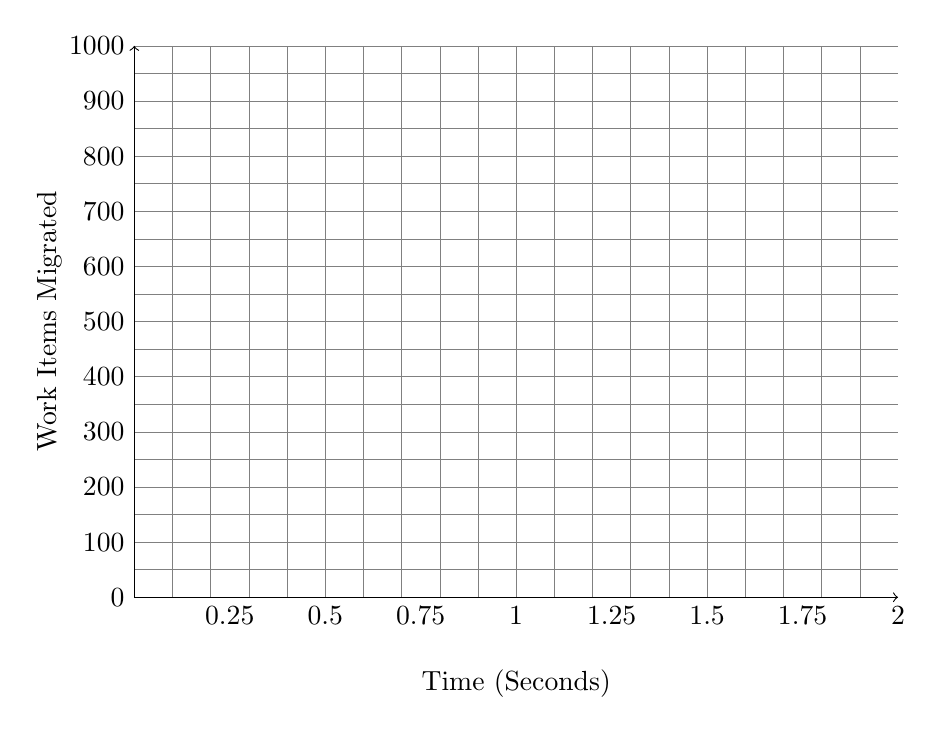
\begin{tikzpicture}[only marks,x=0.4\textwidth,y=0.007cm]

  \def\xmin{0}
  \def\xmax{2}
  \def\ymin{0}
  \def\ymax{1000}

  % grid
  \draw[style=help lines, ystep=50, xstep=0.1] (\xmin,\ymin) grid (\xmax,\ymax);

  % axes
  \draw[->] (\xmin,\ymin) -- (\xmax,\ymin); % node[right] {$x$};
  \draw[->] (\xmin,\ymin) -- (\xmin,\ymax); % node[above] {$y$};

  %labels      
    \draw (1,0) -- coordinate (x axis mid) (1,0);
	\draw (0,500) -- coordinate (y axis mid) (0,500);
    \node[below=0.8cm] at (x axis mid) {Time (Seconds)};
    \node[rotate=90, above=0.8cm] at (y axis mid) {Work Items Migrated};


  % xticks and yticks
  \foreach \x in {0.25,0.5,...,2}
    \node at (\x, \ymin) [below] {\x};
  \foreach \y in {0,100,...,1000}
    \node at (\xmin,\y) [left] {\y};

% ALL PLOTS. Might make things a little clearer.
    \draw[color=gray] plot[mark=*,mark size=0.5pt] file {results/laptrace1/all.data};

    \draw[color=black] plot[mark=*,mark size=0.8pt] file {results/laptrace1/tid0.data};
%    node [right] {thread 0};
%    \draw[color=green] plot[mark=*,mark size=0.7pt] file {results/laptrace1/tid1.data};
%    node [right] {thread 1};
%    \draw[color=red] plot[mark=*,mark size=0.7pt] file {results/laptrace1/tid2.data};
%    node [right] {thread 2};
%    \draw[color=yellow] plot[mark=*,mark size=0.7pt] file {results/laptrace1/tid3.data};
%    node [right] {thread 3};
%    \draw[color=purple] plot[mark=*,mark size=0.7pt] file {results/laptrace1/tid4.data};

\end{tikzpicture}

% full caption
\caption{
    A scatter plot where each point is a succesful steal operation.
    Each point is a mapping of time of occurance, and frequency of work items migrated in the operation.
    Points marked in black are collected from a single run of the program. Gray points are extracted from an additional four runs.
    All data is collected using trace mode two documented in section \ref{sec:traceimp}, where the raster plane is ten-thousand
    squared in dimension and the maximum iterations is set to seventy.
}
\label{fig:tracelap1}
\end{figure}
